%%%%%%%%%%%%%%%%%%%%%%%%%%%%%%%%%%%%%%%%%
% FRI Data Science_report LaTeX Template
% Version 1.0 (28/1/2020)
% 
% Jure Demšar (jure.demsar@fri.uni-lj.si)
%
% Based on MicromouseSymp article template by:
% Mathias Legrand (legrand.mathias@gmail.com) 
% With extensive modifications by:
% Antonio Valente (antonio.luis.valente@gmail.com)
%
% License:
% CC BY-NC-SA 3.0 (http://creativecommons.org/licenses/by-nc-sa/3.0/)
%
%%%%%%%%%%%%%%%%%%%%%%%%%%%%%%%%%%%%%%%%%


%----------------------------------------------------------------------------------------
%	PACKAGES AND OTHER DOCUMENT CONFIGURATIONS
%----------------------------------------------------------------------------------------
\documentclass[fleqn,moreauthors,10pt]{ds_report}
\usepackage[english]{babel}
\usepackage{array}

\graphicspath{{fig/}}




%----------------------------------------------------------------------------------------
%	ARTICLE INFORMATION
%----------------------------------------------------------------------------------------

% Header
\JournalInfo{FRI Natural language processing course 2022}

% Interim or final report
\Archive{Project report} 
%\Archive{Final report} 

% Article title
\PaperTitle{Automatic semantic relation extraction} 

% Authors (student competitors) and their info
\Authors{Aljoša Koren, Klemen Škrlj, Tilen Kavčič and Živa Simonišek}

% Advisors
\affiliation{\textit{Advisors: Slavko Žitnik, Špela Vintar}}

% Keywords
\Keywords{Semantic relation extraction, TermFrame knowledge base}
\newcommand{\keywordname}{Keywords}


%----------------------------------------------------------------------------------------
%	ABSTRACT
%----------------------------------------------------------------------------------------

\Abstract{
Relation extraction is a task that requires automatic detection and classification of semantic relations within a sentence. In this paper we use deep learning approaches to extract relations from TermFrame dataset, which consists of definitions of Karst specific expressions in English and Slovene. We use BERT and AGGCN models for classification of entity pairs in relation. Our best performing model is RoBERTa with F-score of 75,9\% on English corpus and 73\% on Slovene. Automatic relation extraction performs best for "Definiendum" and "Genus" classes while other relations are quite hard for our model. Lastly we include manual evaluation of automatic extraction and reasoning behind successful and unsuccessful predictions.
}

%----------------------------------------------------------------------------------------

\begin{document}

% Makes all text pages the same height
\flushbottom 

% Print the title and abstract box
\maketitle 

% Removes page numbering from the first page
\thispagestyle{empty} 

%----------------------------------------------------------------------------------------
%	ARTICLE CONTENTS
%----------------------------------------------------------------------------------------


\section{Introduction}
Various natural language processing techniques have been proposed to tackle relation extraction. These techniques are most often shown on broad language corpora like the New York Times corpus~\cite{sandhaus2008new} and are trained and tested in the most common languages, most often English. In this paper we focus on the Karstology domain, with sentences in Slovenian and English. Sentences used for model training are hand annotated by linguists. We explore how we can use current natural language techniques to extract both hypernym---hyponym pairs and more non-hierarchical semantic relations.  Since our goal is that our methods not only work on this very domain-specific corpora, we also test our models on the SemEval2010 Task-8 dataset~\cite{hendrickx-etal-2010-semeval}. 

\section{Related work}
There are usually two types of algorithms for discovering the hyponym-hypernym relation; pattern-based and distributional methods. The pattern-based approach is usually time-consuming and language dependent, even if we take the same language from a different time period. Distributional methods can be supervised or unsupervised. They use word distribution to extract hypernyms. Roller et al. \cite{DBLP:journals/corr/abs-1806-03191} compared both approaches in 2018. Both approaches use co-occurrences within a context, however pattern-based use predefined manually chosen patterns, while distributional methods use unconstrained word co-occurrences. They have extracted simple Hearst patterns and also broader patterns, took frequency of occurrences and sparsity into account and postpreprocessing which removed pairs that did not occur in enough sentences. This method was discovered to be better then the rest distributional methods they were comparing it with.  
The work done by Atzori and Balloccu~\cite{Atzori2020} used a unsupervised learning for hypernym discovery. They used cosine distance in vector word embeddings as it was done before, but they added rank weighted by word frequencies in a corpus and level of similarity, to remove the semantic relations that might not be in the hyponym-hypernym relation. Their system is domain and language independent, because they do not use Hearst patterns~\cite{hearst-1992-automatic} (realtions of the form x is-a y) or stopwords, but solely unstructured data.

Paper \cite{bordea-etal-2016-semeval} describes results of a challenge where competitors had to extract hypernym-hyponym relations between a given list of domain-specific terms. The best approach was based on Hearst patterns where the team made use of large web corpus. The distributional approaches got competitive recall but struggled with precision. In a competition \cite{camacho-collados-etal-2018-semeval} teams were presented with a task of finding suitable hypernyms of a given word from the target corpus. The corpuses were multilingual and also domain-specific. Here, a system that learned embeddings of hyponym-hypernym pairs combined with unsupervised learning of Hearst-style patterns performed the best. Overall, supervised methods showed clear superiority over unsupervised ones.

Dependency trees are commonly used to tackle extraction of new intra-sentence instances of semantic relations. To keep only the most relevant information pruning is used. Zhijiang Guo , Yan Zhang and Wei Lu (2019)~\cite{zhijiang_nodate}, for example, introduce Attention Guided Graph Convolutional Networks s (AGGCNs) which use a soft-pruning approach to clean up the dependency tree and keep the relevant sub-structures useful for the relation extraction task. AGGCNs transform the dependency tree into a fully connected edge-weighted graph. Weights represent the relatedness between nodes. They achive 69\% F-score in TACRED dataset on sentence level relation classification. Since dependency trees don’t capture inter-sentence relations, recurrent neural networks (RNNs) and convolutional neural networks (CNNs) are often used. Sahu et al. 2019~\cite{sunil_kumar_nodate} employ their edge Graph CNN (GCNN) model to capture local and non-local dependencies. The graph nodes represent words while edges correspond to semantic dependencies. They use MIL-based bi-affine pairwise scoring function to infer relations between entities from the entity node representations. 

BERT-based pre-training model with cascade tagging framework was first used by Kang Zhaoab et al.~\cite{wei2019novel}. They used their cascade binary tagging framework in which in order to solve the problem of multiple overlapping triplets present in the same sentence share the same entities.  When employing a pre-trained BERT encoder their model achieved F1 score of  89.6 on the NYT dataset and 91.8 on the WebNLG dataset. 

Kang Zhaoab et al.~\cite{ZHAO2021106888} build on this work by introducing graph neural networks. They represent the words as nodes on the graphs and iteratively fuse two types of semantic nodes using the message passing mechanism. With this method they managed to improve the F1 score on the NYT dataset to 92.0 and WebNLB to 92.6. Their model managed to perform on par to the state-of-the-art on the SemEval-2010 Task 8, with the F1 score of 91.3. 

The state-of-the-art on this relation extraction task is the QA model by Amir DN Cohen, Shachar Rosenman and Yoav Goldberg~\cite{cohen2020relation}. They approach the task as a span-prediction problem, which besides on the SemEval-2010 Task 8 also achieves state-of-the-art results on the TACRED dataset. Instead of formulating the problem as a relation classification task, where a sample encompasses a sentence, two head and tail entities and relation. Span Prediction, however formulates the problem using only a sentence, query and an answer to the query. They then use BERT to achieve F1 score of 91.9 on the SemEval-2010 Task 8.


%------------------------------------------------

\section{Methods}
\subsection{BERT}
\par As for the first method we implemented relation extraction with BERT  \cite{BERT:DBLP:journals/corr/abs-1810-04805}. BERT is a transformer-based pre-trained model, designed to pre-train bidirectional representations from unlabeled text by jointly conditioning on both left and right context in all layers. Firstly we marked the continuous words that describe this relationships with special characters. We marked their relationship with one of the chosen relationships and we also marked the position. If the definiendum occurred after the genus, we would mark it with a different class than if it occurred before it. At the end the model had a linear layer predicting 14 classes in total. The sentences were firstly tokenized using pretrained model and the classes were encoded into numbers. The sentences were input into pretrained BERT model and then the output was fed into a linear layer. We used Adam optimizer and a cross entropy loss function. We fine-tuned the pretrained model on the domain dataset and tested the performance. We tried using BERT \cite{BERT:DBLP:journals/corr/abs-1810-04805}, DistilBERT \cite{distiledBert:DBLP:journals/corr/abs-1910-01108} and RoBERTa \cite{roberta:DBLP:journals/corr/abs-1907-11692} and CroSloEngual BERT \cite{ulcar-robnik2020finest}. The main differences between models are that RoBERTa was trained on 10 times more data than BERT, while DistilBERT uses only half the number of parameters. CroSloEngual BERT was trained only on three languages (Croatian, Slovenian and English) and therefore better than a multilingual BERT model on tasks in this three languages. 

\par We also use BERT model for token classification in order to extract relations from un-annotated sentences. For training our model we input tokenized sentences that are POS tagged with the use of Stanza library\textsuperscript{\cite{qi2020stanza}}. Additionally we mark all tokens that we want to classify with their labels. If we look at for example definiendum we mark start token with "B-DEFINIENDUM" and all other tokens that are part of this group with "I-DEFINIENDUM". This is standard way of data representation for our pretrained model. We try different models and training schemes to obtain the best possible results on English and Slovene data. 


\subsection{Attention Guided Graph Convolutional Network}
\par For our second method we use Attention Guided Graph Convolutional Network model, which is described in paper \cite{zhijiang_nodate}. The dependency trees generated from sentences convey rich structural information that is proven useful for relationship extraction from text. However, they also include many irrelevant information that do not help in our task. To automate solution for this problem, authors use novel attention based GNN architecture, which learns important dependencies through "soft-pruning" the tree. 
\par The model consists of three main layers as seen on Figure \ref{fig:aggcn}. The first one is Attention Guided layer. Here the input is adjacency matrix of dependency graph. Through multi headed attention, the network is transformed into N fully connected graph where numbers in the new adjacency matrices represent weights of the edges. This tries to encode which links are important for relation extraction. Each output is then fed into a set of Densely Connected layers. With this the model captures more structural information from these new larger graphs. Resulting feature vector has rich local and non-local information about the sentence. Lastly all N feature vectors are concatenated and fed into linear combination layer which finally predicts the appropriate relationship type.

\begin{figure}[h]
    \centering
    \includegraphics[width=1\columnwidth]{images/AGGCN.png}
    \caption{AGGCN model arhitecture \textsuperscript{\cite{zhijiang_nodate}}}
    \label{fig:aggcn}
\end{figure}

\newpage
\par This model is based on dependency graphs so we need to generate it for each sentence that we want to use. For this we use Stanza library \textsuperscript{\cite{qi2020stanza}}. Additionally we also tokenize each sentence, perform POS tagging and mark which tokens represent object and subject of the relation. Because the given Karst dataset is not perfect, we have to also define some edge cases when we are matching the right object and subject inside given sentence. After that a vocabulary is created. We download GloVe word embedding\textsuperscript{\cite{pennington2014glove}} and find the most possible amount of matches for our vocabulary. This produces 300 dimensional vector for each one of our matched words. Together with previously acquired dependency graphs, POS tags and locations of object/subjects this represents the input to the model. 


%------------------------------------------------

\section{Evaluation}
\subsection{Data}
\par Our primary dataset is TermFrame knowledge base\textsuperscript{\cite{Vintar2019ModellingSK}} which is a Karstology domain specific corpora for three languages; Slovenian, English and Croatian. In Table \ref{tab:karst} we see that the whole corpora is 157 documents in total which were scrapped from various web sources and then hand annotated by linguists. 

\begin{table}[h]
\begin{center}
    \begin{tabular}{ |c|| c| c | c |} 
      \hline
       & \textbf{English} & \textbf{Slovene} & \textbf{Croatian} \\ 
      \hline \hline
      \textbf{Tokens} & 2,721,042  & 1,208,240 & 1,229,368 \\ 
      \hline
      \textbf{Words} & 2,195,982  & 987,801 & 969,735 \\ 
      \hline
      \textbf{Sentences} & 97,187 & 51,990 & 53,017 \\ 
      \hline
      \textbf{Documents} & 57  & 60 & 43 \\ 
      \hline
    \end{tabular}
    \caption{The TermFrame corpora information.}
    \label{tab:karst}
\end{center}
\end{table}

\par TermFrame corpus is annotated with 5 informations: canonical form, semantic category, definition element, semantic relation and relation definitor. Definition element gives us information about definiendum. Definiendum is the term which is defined in the definition sentence. We then tried to define relationships that are connected to it. There are 16 original relations in total: Genus, Has\_size, Has\_location, Has\_cause, Affects, etc., but we also have to take into account reverse relations where definiendum is after relation. This doubles the total number of classes. Some of them have very few appearances in the corpus, so we didn't use them in all of our models, since there isn't enough data to learn on. At the end we focused on 7 most frequent relationships (Genus, Has\_form, Has\_location, Has\_cause, Composition\_medium, Has\_size, and Has\_function). We present number and frequency of occurrences for each of these classes in Table \ref{tab:karst_classes}. Counting every Definiendum-Relation pair separately there are 2641 of them in English part of the corpus and 2706 in Slovene.

\begin{table}[h]
    \centering
    \begin{tabular}{|c|c|c|c|c|}
    \hline
        \textbf{Relation name} & \multicolumn{2}{|c|}{\textbf{\# Occurances}} & \multicolumn{2}{|c|}{\textbf{Frequency}} \\
        & EN & SL & EN & SL \\
        
        \hline \hline
        Genus & 619 & 643 & 29.7\% & 32.2\% \\ \hline
        Genus\_rev & 81 & 112 & 3.9\% & 5.6\% \\ \hline
        Has\_form & 347 & 292 & 16.7\% & 14.6\% \\ \hline
        Has\_form\_rev & 53 & 28 & 2.5\% & 1.4\% \\ \hline
        Has\_location & 325 & 311 & 15.6\% & 15.6\% \\ \hline
        Has\_location\_rev & 26 & 34 & 1.2\% & 1.7\% \\ \hline
        Has\_cause & 201 & 208 & 9.6\% & 10.4\% \\ \hline
        Has\_cause\_rev & 22 & 14 & 1.1\% & 0.7\% \\ \hline
        Comp\_medium \footnotemark[1] & 143 & 95 & 6.9\% & 4.8\% \\ \hline
        Comp\_medium\_rev \footnotemark[2] & 30 & 8 & 1.4\% & 0.4\% \\ \hline
        Has\_size & 117 & 103 & 5.6\% & 5.2\% \\ \hline
        Has\_size\_rev & 12 & 10 & 0.6\% & 0.5\% \\ \hline
        Has\_function & 95 & 131 & 4.6\% & 6.6\% \\ \hline
        Has\_function\_rev & 13 & 11 & 0.6\% & 0.6\% \\ \hline
    \end{tabular}
    \caption{Karst train dataset semantic relations}
    \label{tab:karst_classes}
\end{table}

\footnotetext[1]{Abbreviation for Composition\_medium}
\footnotetext[2]{Abbreviation for Composition\_medium\_rev}


\par As our second dataset, to test our models on, we choose SemEval2010 Task-8 dataset as described in paper \cite{hendrickx-etal-2010-semeval}. It was designed as a benchmark dataset for semantic relation classification in the SemEval competition. The whole corpora contains 10717 sentences with around 200 thousand tokens in total. The goal is to classify noun pairs into one of 11 relations. In Table \ref{tab:semeval} we see total number and frequency of occurrences for each relation. We can notice that there are no reverse relations in this dataset.

\begin{table}[h]
    \centering
    \begin{tabular}{|c|c|c|}
    \hline
        \textbf{Relation name} & \textbf{\# Occurrences} & \textbf{Frequency} \\ \hline \hline
        Cause-Effect & 1331 & 12.4\% \\ \hline
        Component-Whole & 1253 & 11.7\% \\ \hline
        Entity-Destination & 1137 & 10.6\% \\ \hline
        Entity-Origin & 974 & 9.1\% \\ \hline
        Product-Producer & 948 & 8.8\% \\ \hline
        Member-Collection & 923 & 8.6\% \\ \hline
        Message-Topic & 895 & 8.4\% \\ \hline
        Content-Container & 732 & 6.8\% \\ \hline
        Instrument-Agency & 660 & 6.2\% \\ \hline
        Other & 1864 & 17.4\% \\ \hline
    \end{tabular}
    \caption{SemEval2010 Task 8 dataset semantic relations}
    \label{tab:semeval}
\end{table}


\subsection{Performance metrics}
\par Our main goal for this task is classifying word pairs into proper relation. Because of that we use standard classification performance metrics to evaluate and compare our models. We calculate precision, recall and then F-score which is used as a main metric to evaluate how good the model is. Since this is a multi-classification problem and classes are imbalanced we have to calculate measures for each class separately. And because all the classes are equally important we take the unweighted average over all the scores as our final performance. 
\par We also need to evaluate relationship extraction. Similarly to word pair classification problem, we can here also use metrics mentioned above. For each word that is tagged as some relation we check if the tag is correct. Based on this precision, recall and F-score are again calculated per tag class and averaged together. 


%------------------------------------------------

\section{Results}

\subsection{Relation classification}
\par In the first part we tested how good are our models on a task of classifying an object-subject pair into correct relation. We train our AGGCN model for 150 epochs with SGD optimizer, starting learning rate of 0.5 and 0.9 weight decay every fifth epoch. Architecture uses 3 attention heads and batch size of 50. BERT models were fine-tuned on just 5 epochs. Adam optimizer was used with a learning rate of 2e-05 and batch size of 16. 

\par Firstly, we test our models on SemEval dataset. In Table \ref{tab:semeval_aggcn} we see AGGCN performance per class and its overall score. We also test three different versions of BERT models on the same dataset and look at their overall performance in Table \ref{tab:semeval_bert}. From this results we see that RoBERTa worked the best, as it was expected for the biggest model. We decided to use it as it performed the best on a similar task.

\begin{table}[h]
    \centering
    \begin{tabular}{|c|c|c|c|}
        \hline
        \textbf{Relation name} & \textbf{Prec} & \textbf{Rec} & \textbf{F-score} \\ \hline \hline
        Cause-Effect        &  0.918  &  0.923  &  0.921 \\ \hline
        Component-Whole     &  0.829  &  0.826  &  0.828 \\ \hline
        Content-Container   &  0.824  &  0.880  &  0.851 \\ \hline
        Entity-Destination  &  0.865  &  0.924  &  0.894 \\ \hline
        Entity-Origin       &  0.827  &  0.856  &  0.841 \\ \hline
        Instrument-Agency   &  0.794  &  0.769  &  0.781 \\ \hline
        Member-Collection   &  0.835  &  0.871  &  0.852 \\ \hline
        Message-Topic       &  0.823  &  0.911  &  0.865 \\ \hline
        Product-Producer    &  0.822  &  0.861  &  0.841 \\ \hline \hline
        \textbf{Overall performance} & 0.838 & 0.870 & 0.853 \\ \hline
    \end{tabular}
    \caption{Results of AGGCN model on SemEval dataset}
    \label{tab:semeval_aggcn}
\end{table}

\begin{table}[h]
    \centering
    \begin{tabular}{|c|c|c|c|}
        \hline
        \textbf{Model name} & \textbf{Prec} & \textbf{Rec} & \textbf{F-score} \\ \hline \hline
        BERT        &  0.808  &  0.825  &  0.800 \\ \hline
        DistilBERT     &  0.803  &  0.815  &  0.793 \\ \hline
        \textbf{RoBERTa}   &  \textbf{0.817}  & \textbf{0.823}  &  \textbf{0.803} \\ \hline
        CroSloEngual   &  0.790  &  0.814  &  0.782 \\ \hline
    \end{tabular}
    \caption{Overall results of different BERT models on SemEval dataset}
    \label{tab:semeval_bert}
\end{table}

\par After that we train and evaluate AGGCN model on English part of TermFrame dataset. Table \ref{tab:karst_all} shows overall results when predicting all available classes (32 of them). We also compare this results to classifications of our BERT model.

\begin{table}[h]
    \centering
    \begin{tabular}{|c|c|c|c|}
        \hline
        \textbf{Model name} & \textbf{Prec} & \textbf{Rec} & \textbf{F-score} \\ \hline \hline
        \textbf{AGGCN}        &  \textbf{0.319}  &  \textbf{0.272}  &  \textbf{0.294} \\ \hline
        RoBERTa     &  0.263  &  0.226  &  0.243 \\ \hline
    \end{tabular}
    \caption{Overall results when classifying all TermFrame EN classes}
    \label{tab:karst_all}
\end{table}

\newpage
\par When we closely inspect which classes cause the most amount of problems we see the expected results. Some of them are "Affects", "Measures", "Occures in time", etc. This are also the classes that are underrepresented in our training set.

\par This is why we then train and test classification models just on a subset of most frequently occurring classes as seen in Table \ref{tab:karst_classes}. In Table \ref{tab:karst_subset} we can see per class and overall performance of AGGCN classificator on an EN TermFrame corpus. We can see that the test set doesn't include reverse relations so they are omitted from the results. Genus relations are the easiest to classify which is expected since in many sentences there are "is-a" or other similar patterns that connect definiendum and genus. On the other hand, our model has a lot of trouble with false negative predictions of "Has\_function" relation which is shown in very low recall and subsequently low F-score.

\begin{table}[!ht]
    \centering
    \begin{tabular}{|c|c|c|c|}
        \hline
        \textbf{Relation name} & \textbf{Prec} & \textbf{Rec} & \textbf{F-score} \\ \hline \hline
        Composition\_medium  &  0.764  &  0.500  &  0.604 \\ \hline
        Genus               &  0.834  &  0.982  &  0.902 \\ \hline
        Has\_cause           &  0.655  &  0.542  &  0.593 \\ \hline
        Has\_form           &  0.538  &  0.636  &  0.583 \\ \hline
        Has\_function        & 1  &   0.071  &  0.133 \\ \hline
        Has\_location        &  0.435  &  0.566  &  0.492 \\ \hline
        Has\_size            & 1 &  0.642  &  0.782 \\ \hline \hline
        \textbf{Overall performance} & 0.750 & 0.563 & 0.642 \\ \hline
    \end{tabular}
    \caption{Results of AGGCN model on EN TermFrame (using subset of all classes)}
    \label{tab:karst_subset}
\end{table}


\par We do the same evaluation by training and testing RoBERTa model on English part of TermFrame dataset and present results in Table \ref{tab:karst_subset_bert}. Genus and Has\_size relations are learned the best while similarly to AGGCN this model also has the most amount of trouble with Has\_function relation.

\begin{table}[!ht]
    \centering
    \begin{tabular}{|c|c|c|c|}
        \hline
        \textbf{Relation name} & \textbf{Prec} & \textbf{Rec} & \textbf{F-score} \\ \hline \hline
        Composition\_medium  &  0.857  &  0.619  &  0.698 \\ \hline
        Genus               &  1  &  0.991  &  0.995 \\ \hline
        Has\_cause           &  0.9  &  0.633  &  0.716 \\ \hline
        Has\_form           &  0.941  &  0.765  &  0.829 \\ \hline
        Has\_function        & 0.357  &   0.286  &  0.310 \\ \hline
        Has\_location        &  0.923  &  0.615  &  0.695 \\ \hline
        Has\_size            & 0.923 &  0.923  &  0.923 \\ \hline \hline
        \textbf{Overall performance} & 0.843 & 0.690 & 0.759 \\ \hline
    \end{tabular}
    \caption{Results of RoBERTa model on EN TermFrame (using subset of all classes)}
    \label{tab:karst_subset_bert}
\end{table}



\par From our results on SemEval and English part of TermFrame datasets we see that RoBERTa gave us comparable or much better performance compared to AGGCN so this is what we used going forward. 
\par In Table \ref{tab:karst_subset2_en_sl} we see results of RoBERTa and CroSloEngual versions of BERT model trained and tested on Slovene corpus. We can see that CroSloEngual majorly outperforms RoBERTa. This is expected as multilingual models perform worse than monolingual or in our case trilingual models. 

\begin{table}[!ht]
    \centering
    \begin{tabular}{|c|c | c|c | c|c | c|}
        \hline
        \textbf{Relation} & \multicolumn{2}{|c|}{\textbf{Prec}} & \multicolumn{2}{|c|}{\textbf{Rec}} & \multicolumn{2}{|c|}{\textbf{F-score}} \\ \hline \hline
        &  R & C &  R  & C &  R & C\\ \hline
        CM \footnotemark[1]  & 0.0 & 0.83 & 0.0 & 0.83 & 0.0 & 0.83 \\ \hline
        CM\_rev \footnotemark[2]  & 0.0  & 1 & 0.0 & 1 & 0.0 & 1 \\ \hline
        G               & 0.93  & 0.99 & 0.66  & 0.91 & 0.75 &  0.94\\ \hline
        G\_rev               & 0.97 & 1 & 0.90  & 0.97 & 0.93 &  0.98\\ \hline
        HS           &  0.56 & 0.89 &  0.39 &  0.72 &  0.44 & 0.78\\ \hline
        HS\_rev           &  0.0 & 0.50 &  0.0 &  0.25 &  0.0 & 0.33\\ \hline
        HF           &  0.97 & 1 &  0.62 & 0.85 &  0.73 & 0.91 \\ \hline
        HF\_rev           &  0.0 & 0.50 &  0.0 & 0.38 &  0.0 & 0.42 \\ \hline
        HFun       & 0.0  & 0.67 &  0.0 & 0.67 &  0.0 & 0.67 \\ \hline
        HFun\_rev        & /  & / &  / & / &  / & / \\ \hline
        HL        &  0.87  & 1 & 0.74 & 0.78 &  0.78 & 0.86 \\ \hline
        HL\_rev        &  1  & 1 & 0.5 & 1 &  0.63 & 1 \\ \hline
        HS            & 0.0 & 1 & 0.0  & 0.92 & 0.0 & 0.95\\ \hline
        HS\_rev            & 0.0 & 0.0 & 0.0  & 0.0 & 0.0 & 0.0\\ \hline \hline
        \textbf{Overall} & 0.33 & \textbf{0.75} & 0.35 & \textbf{0.74} & 0.32 & \textbf{0.73}\\ \hline
    \end{tabular}
    \caption{Results of RoBERTa (R) and CroSloEngual (C) on Slovene TermFrame (using subset of all classes)}
    \label{tab:karst_subset2_en_sl}
\end{table}

We also tried using CroSloEngual as a zero shot learning model. We fine-tuned the model on English TermFrame dataset and then tested it on the Slovenian test set. It achieved the overall precision of 0.685, recall of 0.682 and the F1-score of 0.658. We can see that the model performed worse than when it was also fine-tuned on the Slovenian corpus. However, the results were not the worst. This means that the model learns how the relations are formed which can be transferred in both languages.


\subsubsection{Visualization of semantic network}
For the classification task we also made a visualization network. We made connections between pairs of nodes we were classifying. Nodes contain the subsentences that we are classifying, while the links contain the predicted class. If the classifier predicted the wrong class we denoted this link with the red color. In case the classifier predicted the right class we marked the connection with a black color.
\begin{figure}[h]
    \centering
    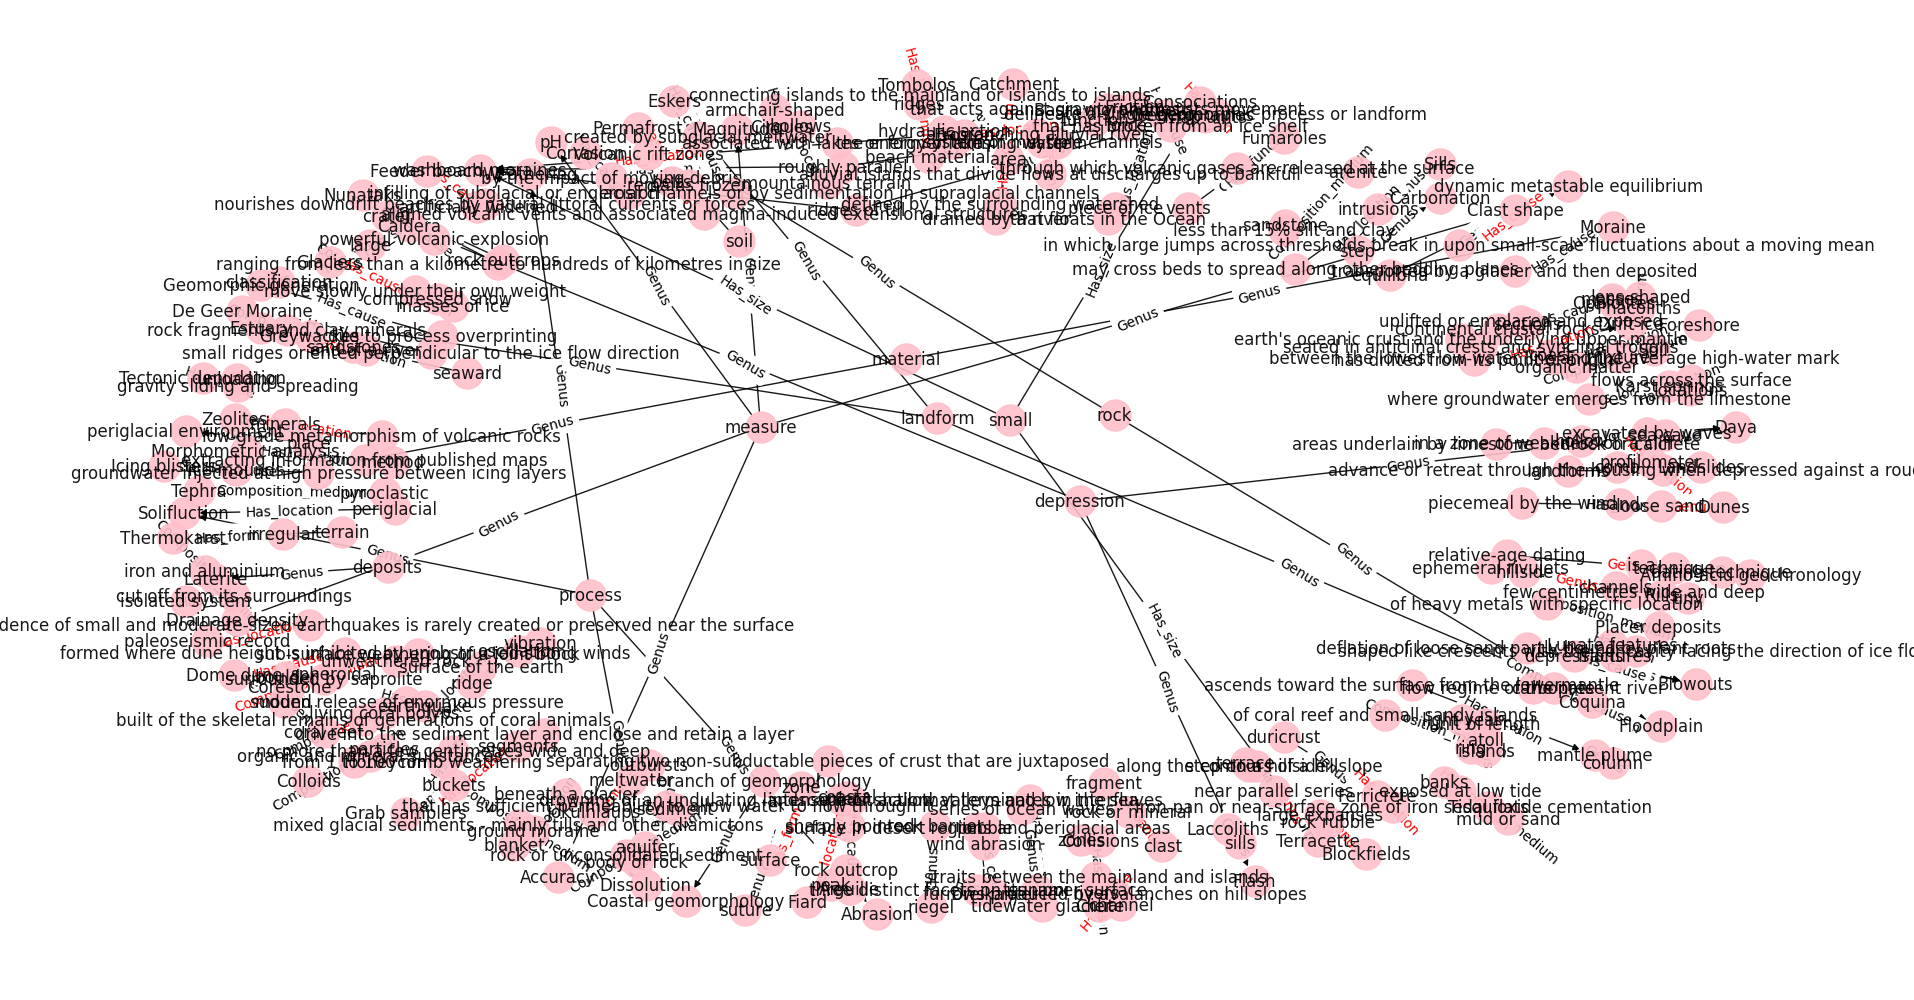
\includegraphics[width=1\columnwidth]{network_vis.png}
    \caption{Whole semantic network.}
    \label{fig:sem_net1}
\end{figure}
\begin{figure}[h]
    \centering
    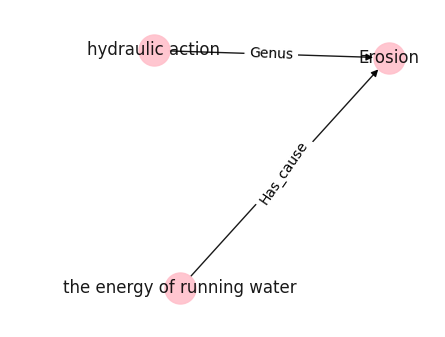
\includegraphics[width=0.6\columnwidth]{network_vis2.png}
    \caption{A part of the semantic network.}
    \label{fig:sem_net2}
\end{figure}


\subsection{Relation extraction}
\par In the second part of our task we focus on extracting relations from an un-annotated sentence and classifying them into the right labels. In our first pipeline we train our model on English part of Karst corpus. As discussed before, some classes are severely underrepresented so we are only focusing on predicting the ones listed in Table\ref{tab:karst_classes} with addition to "DEFINIENDUM" class. 
\par In Table \ref{tab:tagger_all} we can see results of BERT token classificator evaluated on test dataset. Our model is quite good at labeling definiendum and genus while other classes do not have such good results. One of the reasons for such results for other classes is that this are normally multi-word relations and are thus harder for the model to learn. It seems that the model is not able to capture full meaning for such long representations. The other possible problem is that defininendum and genus are the the most common classes in train and test set by a big margin. The performance would definitely improve if we had more data. This is also confirmed by looking at weighted results where our model gets F-score of 56\%.
\par Additionally we also trained and evaluated models for each relation separately e.g. model that only labels Definiendum and Has\_cause or only Definiendum and Has\_form. We hypothesized that the results would be better if our model focuses only on one relation at a time, but we saw that performance was only slightly improved and in some cases even decreased. This approach would additionally come with problem of overlapping tags where a token could be classified into more classes. Because of this we abandoned this idea.

\begin{table}[!ht]
    \centering
    \begin{tabular}{|c|c|c|c|}
        \hline
        \textbf{Token tag} & \textbf{Prec} & \textbf{Rec} & \textbf{F-score} \\ \hline \hline
        Composition\_medium  &  0.06  &  0.06  &  0.06 \\ \hline
        Definiendum               &  0.91  &  0.95  &  0.93 \\ \hline
        Genus               &  0.44  &  0.47  &  0.46 \\ \hline
        Has\_cause           &  0.06  &  0.06  &  0.06 \\ \hline
        Has\_form           &  0.14  &  0.38  &  0.21 \\ \hline
        Has\_function        & 0.03  &   0.05  &  0.04 \\ \hline
        Has\_location        &  0.06  &  0.08  &  0.07 \\ \hline
        Has\_size            & 0.20 &  0.31  &  0.24 \\ \hline \hline
        \textbf{Overall performance} & 0.24 & 0.29 & 0.26 \\ \hline
    \end{tabular}
    \caption{BERT token classification on EN TermFrame}
    \label{tab:tagger_all}
\end{table}


\par Similarly as with English, we also train and evaluate BERT Token Classificator on Slovene TermFrame corpus. We see results for all tokens in Table \ref{tab:tagger_all_slo}. In test dataset for Slovene corpus we also have some reverse relations and those were very problematic for our model since it can't identify even one true positive token.

\begin{table}[!ht]
    \centering
    \begin{tabular}{|c|c|c|c|}
        \hline
        \textbf{Token tag} & \textbf{Prec} & \textbf{Rec} & \textbf{F-score} \\ \hline \hline
        Composition\_medium  &  0  &  0  &  0 \\ \hline
        Composition\_medium\_rev  &  0  &  0  &  0 \\ \hline
        Definiendum               &  0.78  &  0.79  &  0.79 \\ \hline
        Genus               &  0.62  &  0.59  &  0.61 \\ \hline
        Genus\_rev               &  0.21  &  0.15  &  0.17 \\ \hline
        Has\_cause           &  0.04  &  0.06  &  0.04 \\ \hline
        Has\_cause\_rev           &  0  &  0  &  0 \\ \hline
        Has\_form           &  0.41  &  0.34  &  0.37 \\ \hline
        Has\_form\_rev           &  0  &  0  &  0 \\ \hline
        Has\_function        & 0  &   0  &  0 \\ \hline
        Has\_function\_rev        & 0  &   0  &  0 \\ \hline
        Has\_location        &  0.31  &  0.34  &  0.32 \\ \hline
        Has\_location\_rev        &  0  &  0  &  0 \\ \hline
        Has\_size            & 0.14 &  0.08  &  0.11 \\ \hline
        Has\_size\_rev            & 0 &  0  &  0 \\ \hline \hline
        \textbf{Overall performance} & 0.17 & 0.16 & 0.16 \\ \hline
    \end{tabular}
    \caption{BERT token classification on SL TermFrame}
    \label{tab:tagger_all_slo}
\end{table}


%------------------------------------------------

\subsubsection{Relation extraction manual evaluation}
Manual evaluation of the results was performed by a linguist. For the manual evaluation, the linguist selected 30 test sentences for Slovene and 30 test sentences for English. The linguist evaluated only the team’s predictions and did not mark recall. It was also taken into account that the model’s prediction is correct in some cases when the linguist team annotated the definition differently.

Each prediction was evaluated from two perspectives: if the predicted tag is correct ("Correct") and if the model correctly identified the whole phrase ("Correct phrase"). If any of the two columns was correct, the linguist marked it with a 1 (incorrect tag was marked with 0). For phrases, only the beginning of the phrase was marked with a 1, meaning that the whole phrase is correct.

The predictions for definienda and genera are more accurate than the predictions for semantic relations. In English, 25 out of 29 predicted definienda and 28 out of 43 predicted genera were marked as correct phrases as seen in detail in Table \ref{tab:linguist_en}. 

\begin{table}[!h]
    \centering
    \begin{tabular}{|c|c|c|} \hline
        \textbf{Relation} & \textbf{\# Predicted} & \textbf{\# Correct}\\ \hline
        Has\_Location &26 &12  \\ \hline
        Has\_Size & 8& 8 \\ \hline
        Has\_Function & 4& 0 \\ \hline
        Has\_Form & 30& 13 \\ \hline
        Has\_Cause & 26& 5 \\ \hline
        Composition\_medium & 12& 0 \\ \hline
    \end{tabular}
    \caption{Results on EN corpus after manual check}
    \label{tab:linguist_en}
\end{table}

In Slovene, 23 out of 32 predicted definienda and 16 out of 25 predicted genera were marked as correct phrases. In some cases, the definiendum/genus was not recognized or the sentence had no definiendum/genus. Full results are seen in Table \ref{tab:linguist_sl}.

\begin{table}[!h]
    \centering
    \begin{tabular}{|c|c|c|} \hline
        \textbf{Relation} & \textbf{\# Predicted} & \textbf{\# Correct}\\ \hline
        Has\_Location &19 &11  \\ \hline
        Has\_Size & 3& 2 \\ \hline
        Has\_Function & 11& 0 \\ \hline
        Has\_Form & 19& 8 \\ \hline
        Has\_Cause & 14& 9 \\ \hline
        Composition\_medium & 7& 0 \\ \hline
    \end{tabular}
    \caption{Results on SL corpus after manual check}
    \label{tab:linguist_sl}
\end{table}

The model was most successful in predicting semantic relation HAS\_SIZE in both languages, followed by \\ HAS\_LOCATION in English and HAS\_CAUSE in Slovene.

Only six semantic relations were selected for the model and this resulted in some better predictions. On the other hand, this is also the reason why some relations were predicted incorrectly: \emph{V geologiji je zemeljski plaz definiran kot območje preperine, usedline ali kamnine, ki se je hitro ali počasi premaknila s prvotnega kraja in ima vidno spremenjeno površje.}
This part \emph{"ima vidno spremenjeno površje"} was previously annotated by the linguist team as HAS\_RESULT. The model predicted this part of the sentence as a mixture of two relations, HAS\_FUNCTION and HAS\_FORM.

There were some sentences where only the preposition was marked as HAS\_LOCATION: \emph{Takšnim meandrom pravimo tudi ujeti meandri in jih najdemo tudi v nekaterih drugih slovenskih pokrajinah.}
In this sentence, the model has marked the preposition \emph{"v"} as HAS\_LOCATION, which cannot be considered as a correct phrase or a correct tag, as the \emph{"v"} itself has no meaning and does not express a location.

In the next example, the model predicted the semantic relation HAS\_CAUSE (\emph{"dviganju antiklinale vrezal prečno na antiklinalo"}) and did not include the preposition \emph{"ob"}, but the linguist evaluated this as a correct phrase because the omitted preposition does not change the meaning and we can still conclude this is the relation HAS\_CAUSE: \emph{Uporablja se pojem prebojna dolina, kar pa je samo slovenski izraz za antecedentno dolino, to je tisti del rečne doline, ki se je ob dviganju antiklinale vrezal prečno na antiklinalo.}


\section{Discussion}
\par In relation classification task BERT models and also AGGCN perform with F-score between 0.80 and 0.85 on SemEval dataset, while RoBERTa model outperforms AGGCN for 18\% on the English TermFrame dataset. Both performed worst for the classes which were badly represented in the dataset. This is expected as they do not affect a lost function as much as better represented classes. We can also see that models with more parameters perform better on the same dataset. Models that are specifically trained on one language outperform multilingual models in the trained language.   
\par Automatic relation extraction works best for definiendum class where we get F-score of 93\% on English and 79\% on Slovene dataset. After that genus relations are also well extracted while other classes are hard for our models. One of the reasons for such results is definitely number of training examples. Almost all definitions have definiendum-genus relation while other relations are mostly just a byproduct. We also observed that other relations are often composed out of many tokens and since our model is evaluated per token this gives more room for error. This is then confirmed by manual evaluation where some annotations had to be evaluated as wrong since they only contained prepositions and not whole relation.
\par Overall we see that deep learning models can be used as a helping tool to linguists for relation extraction. Currently the best pipeline would be semi-automatic annotation where a model can be used at first and then a human would use predictions as a guide for manual annotation. But with more training examples and better architectures model's reliability can definitely be improved.


%------------------------------------------------

\section{Acknowledgments}
We thank assist. prof. dr. Slavko Žitnik from University of Ljubljana, Faculty of Computer and Information Science for providing guidance through our project, we thank prof. dr. Špela Vintar from University of Ljubljana, Faculty of Arts for explaining the Karst corpus and relationship extraction task and we thank our colleague Živa Simonišek from University of Ljubljana Faculty of Arts for providing manual evaluation.


%----------------------------------------------------------------------------------------
%	REFERENCE LIST
%----------------------------------------------------------------------------------------
\bibliographystyle{unsrt}
\bibliography{report}


\end{document}